\documentclass[14pt]{beamer}
\setbeamertemplate{caption}[numbered]
\setbeamertemplate{caption label separator}{:}
\setbeamercolor{caption name}{fg=normal text.fg}
\usepackage{amssymb,amsmath}
\usepackage{ifxetex,ifluatex}
\usepackage{fixltx2e} % provides \textsubscript
\usepackage{lmodern}
\ifxetex
  \usepackage{fontspec,xltxtra,xunicode}
  \defaultfontfeatures{Mapping=tex-text,Scale=MatchLowercase}
  \newcommand{\euro}{€}
\else
  \ifluatex
    \usepackage{fontspec}
    \defaultfontfeatures{Mapping=tex-text,Scale=MatchLowercase}
    \newcommand{\euro}{€}
  \else
    \usepackage[T1]{fontenc}
    \usepackage[utf8]{inputenc}
      \fi
\fi
% use upquote if available, for straight quotes in verbatim environments
\IfFileExists{upquote.sty}{\usepackage{upquote}}{}
% use microtype if available
\IfFileExists{microtype.sty}{\usepackage{microtype}}{}
\PassOptionsToPackage{hyphens}{url}
\usepackage{hyperref}
\usepackage{ulem}

% Comment these out if you don't want a slide with just the
% part/section/subsection/subsubsection title:
\AtBeginPart{
  \let\insertpartnumber\relax
  \let\partname\relax
  \frame{\partpage}
}
\AtBeginSection{
  \let\insertsectionnumber\relax
  \let\sectionname\relax
  \begin{frame}[plain]
    \tableofcontents[currentsection]
  \end{frame}
}
\AtBeginSubsection{
  \let\insertsubsectionnumber\relax
  \let\subsectionname\relax
  \frame{\subsectionpage}
}

\setlength{\parindent}{0pt}
\setlength{\parskip}{6pt plus 2pt minus 1pt}
\setlength{\emergencystretch}{3em}  % prevent overfull lines
\setcounter{secnumdepth}{0}
% Thanks Richard Darst on how to get a nice Beamer theme.
% See http://rkd.zgib.net/wiki/DebianBeamerThemes

\usepackage{ctable}
\usepackage{multicol}
\usepackage{tikz}
\usetikzlibrary{positioning}

\usebackgroundtemplate{
\includegraphics[width=\paperwidth]{images/swirl-lightest.pdf}}
\logo{
\includegraphics[viewport=274 335 360 440,width=1cm]{images/openlogo-nd.pdf}}

\definecolor{debianred}{rgb}{.780,.000,.211} % 199,0,54
\definecolor{debianblue}{rgb}{0,.208,.780} % 0,53,199
\definecolor{debianlightbackgroundblue}{rgb}{.941,.941,.957} % 240,240,244
\definecolor{debianbackgroundblue}{rgb}{.776,.784,.878} % 198,200,224

\usetheme{Boadilla}
\setbeamertemplate{navigation symbols}{}

\usecolortheme[named=debianbackgroundblue]{structure}
\setbeamercolor{normal text}{fg=black}
\setbeamercolor{titlelike}{fg=debianblue}
\setbeamercolor{sidebar}{fg=debianred,bg=debianbackgroundblue}

\setbeamercolor{palette sidebar primary}{fg=debianred}
\setbeamercolor{palette sidebar secondary}{fg=debianred}
\setbeamercolor{palette sidebar tertiary}{fg=debianred}
\setbeamercolor{palette sidebar quaternary}{fg=debianred}

\setbeamercolor{section in toc}{fg=debianred}
\setbeamercolor{subsection in toc}{parent=debianred}

\setbeamercolor{item}{fg=debianred}

\setbeamercolor{block title}{fg=debianblue}

\title[Reproducible builds]{Stretching out for trustworthy reproducible builds}
\subtitle{Creating bit by bit identical binaries}
\author[Reproducible builds team]{%
   \texorpdfstring{
        Reproducible builds team\\
        \href{mailto:reproducible-builds@lists.alioth.debian.org}{\texttt{reproducible-builds@lists.alioth.debian.org}}
   }{Reproducible builds team}}
\institute[Debian]{}
\date[DebConf15]{%
 DebConf15\\
 \small
 2015-08-20}

\begin{document}

\begin{frame}
 \titlepage
\end{frame}

\begin{frame}
 \begin{center}
  \begin{columns}
   \small
   \column{.33\linewidth}
    akira \\
    Andrew Ayer \\
    Asheesh Laroia \\
    \alt<2>{\alert{Chris Lamb}}{Chris Lamb} \\
    Chris West \\
    Christoph Berg \\
    Daniel Kahn Gillmor \\
    David Suarez \\
    \alt<2>{\alert{Dhole}}{Dhole} \\
    Drew Fisher \\
    Esa Peuha \\
    Guillem Jover
   \column{.33\linewidth}
    Hans-Christoph Steiner \\
    Helmut Grohne \\
    \alt<2>{\alert{Holger Levsen}}{Holger Levsen} \\
    Jelmer Vernooij \\
    josch \\
    Juan Picca \\
    \alt<2>{\alert{Lunar}}{Lunar} \\
    Mathieu Bridon \\
    Mattia Rizzolo \\
    Nicolas Boulenguez \\
    Niels Thykier \\
    Niko Tyni
   \column{.33\linewidth}
    Paul Wise \\
    Peter De Wachter \\
    Philip Rinn \\
    Reiner Herrmann \\
    Stefano Rivera \\
    Stéphane Glondu \\
    Steven Chamberlain \\
    Tom Fitzhenry \\
    Tomasz Buchert \\
    Valentin Lorentz \\
    Wookey \\
    Ximin Luo
  \end{columns}
 \end{center}
\end{frame}

\section{Introduction}

\begin{frame}
 \frametitle{The problem}

 \begin{center}
  \begin{tikzpicture}
   \draw (-2,0) node[font=\LARGE] (source) { source };
   \draw (2,0) node[font=\LARGE] (binary) { binary };
   \draw[->,very thick] (source) -- (binary) node[midway] (midbuild) {};
   \draw (midbuild) node [above,color=debianred,font=\small] (build) {build};
   \visible<2>{
    \draw (0,2) node[font=\LARGE,color=debianblue] (fs) { free software };
    % font= specification is required to work-around a bug in md->latex conversion
    \draw[->,font=\normalsize] (fs) -- (source) node[midway,left=0.2cm,color=debianred,font=\footnotesize,align=center]{freedom\\to study};
    \draw[->,font=\normalsize] (fs) -> (binary) node[midway,right=0.2cm,color=debianred,font=\footnotesize,align=center]{freedom\\to run};
   }
   \visible<3->{
    \draw (-4,-1) node[font=\small,color=debianblue] (verified) { can be verified };
    \draw (4,-1) node[font=\small,color=debianblue] (used) { can be used };
    \path (verified) edge[->,bend left=30] (source);
    \path (used) edge[->,bend right=30] (binary);
   }
   \visible<4->{
    \draw (0,-2) node[font=\LARGE,color=debianred,align=center] (prove) { could I get a proof? };
    \path (prove) edge[->] (midbuild);
   }
  \end{tikzpicture}
 \end{center}
\end{frame}

\begin{frame}[fragile]
 \frametitle{Why does it matter?}

 \begin{center}
  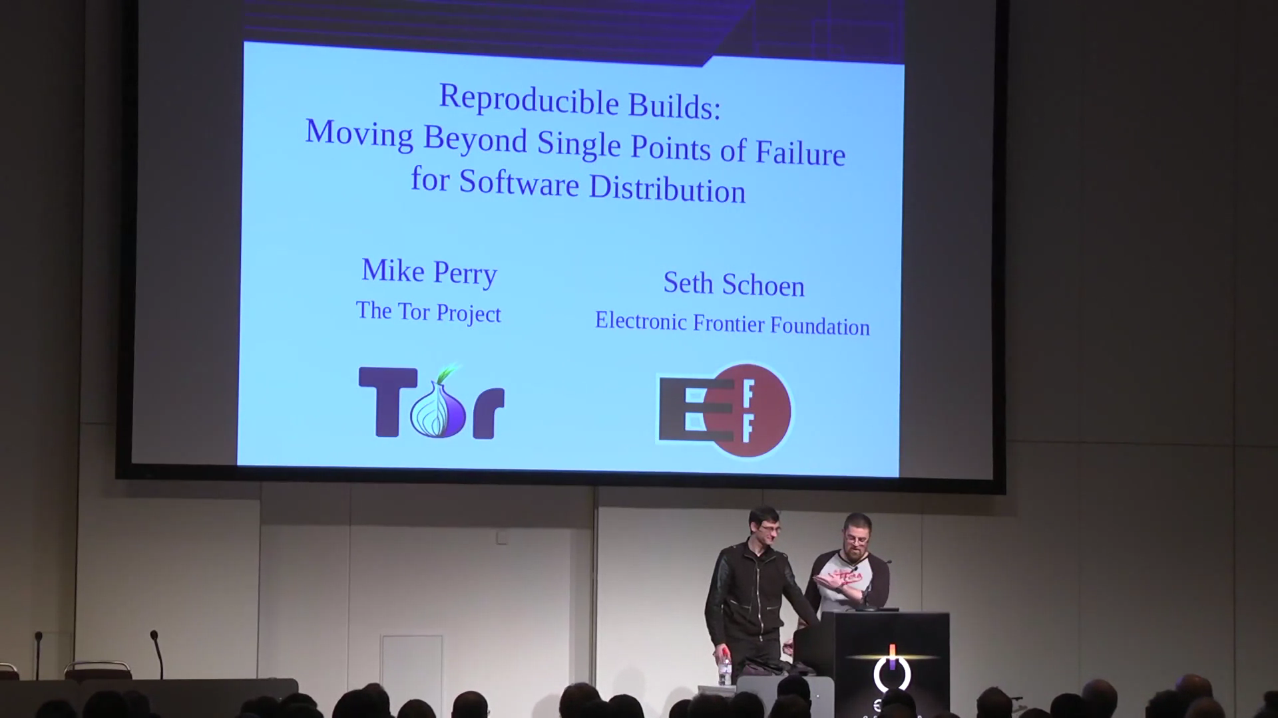
\includegraphics[width=0.7\textwidth]{images/31c3.png}

  Available on \url{media.ccc.de}, 31c3
 \end{center}
\end{frame}

\begin{frame}[fragile]
 \frametitle{Just one example}

 At a CIA conference in 2012:
 \begin{center}
  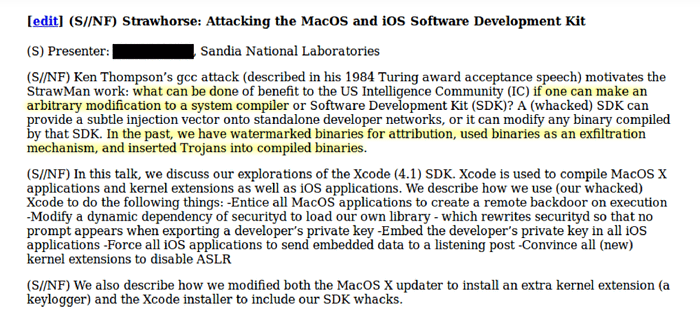
\includegraphics[width=0.8\textwidth]{images/strawhorse.png}

  {\footnotesize
  \url{firstlook.org/theintercept/2015/03/10/ispy-cia-campaign-steal-apples-secrets/}
  }
 \end{center}
\end{frame}

\begin{frame}
 \frametitle{The solution}

 \begin{center}
 \Large
 enable anyone to reproduce\\
 identical binary packages\\
 from a given source
\end{center}

\end{frame}

\begin{frame}
 \frametitle{The solution}

 \begin{center}
 We call this:

 \Huge
 “reproducible builds”
 \end{center}
\end{frame}

\begin{frame}
 \frametitle{It's not only security}

 \begin{itemize}
  \item \texttt{Multi-arch: Same}
  \item Debug packages can be created at any time
  \item Detect FTBFS early
  \item Build profiles
  \item Smaller \texttt{.deb} deltas
  \item Validation of cross-builds
  \item Easier tests of tools
  \item …
 \end{itemize}
\end{frame}

\begin{frame}[plain]
 \begin{tikzpicture}[remember picture,overlay]
  \node[at=(current page.center)] {
    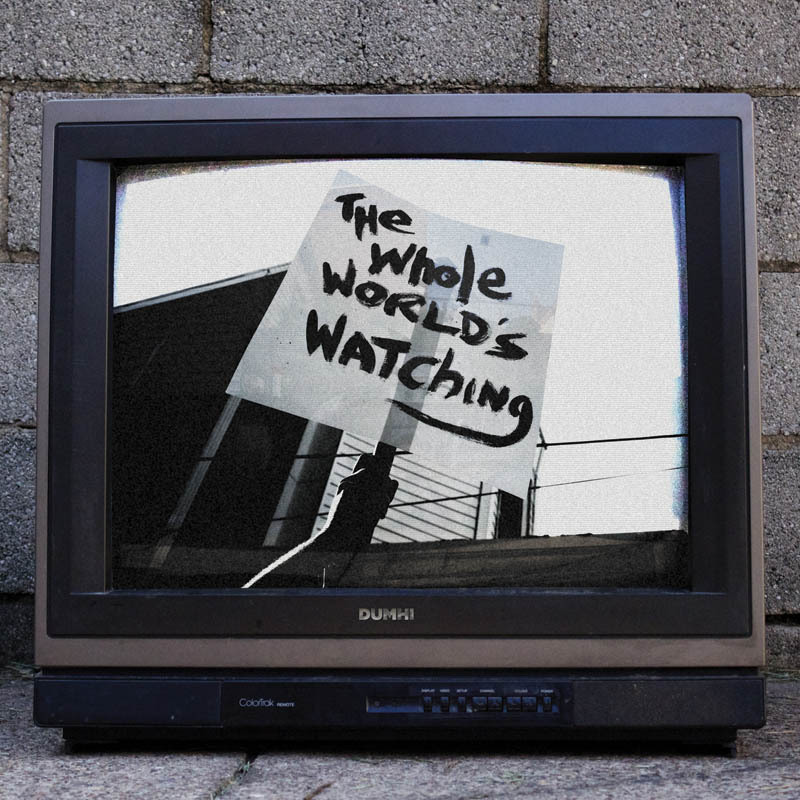
\includegraphics[width=\paperwidth]{images/wholeworld.jpg}
    % Credits to Kevin ‘Chuise’ Jackson
    % http://dumhi.com/about
  };
 \end{tikzpicture}
\end{frame}

\begin{frame}
 \frametitle{So fashionable!}

 \begin{itemize}
 \item Bitcoin (\textbf{done})
 \item Tor (\textbf{done})
 \item Debian (\emph{in progress})
 \item FreeBSD (\emph{in progress})
 \item NetBSD (\emph{in progress})
 \item Coreboot (\textbf{done})
 \item OpenWrt (\emph{in progress})
 \item \ldots{}
\end{itemize}

\end{frame}


\section{Current status}

\begin{frame}
 \frametitle{History}

 \begin{itemize}
  \item Two years!
  \item It's on the wiki:
    {\small \url{https://wiki.debian.org/ReproducibleBuilds/History}}
  \item Weekly reports since May 2015
  \item Many talks already:
   \begin{itemize}
    \item 2014-02-01: FOSDEM’14
    \item 2014-08-26: DebConf14
    \item 2015-01-31: FOSDEM’15
    \item 2015-05-26: Datengarten 52
    \item 2015-06-07: Gulaschprogrammiernacht 15
    \item 2015-06-19: Pas Sage En Seine 2015
    \item 2015-07-06: Libre Software Meeting 2015
    \item 2015-08-13: Chaos Communication Camp 2015
   \end{itemize}
 \end{itemize}
\end{frame}

\begin{frame}
 \frametitle{Since DebConf14}

 \begin{itemize}
  \item \texttt{strip-nondeterminism}
  \item Fixed build path
  \item Recording the build environment: \texttt{.buildinfo}
  \item \texttt{reproducible.debian.net}
  \item \texttt{diffoscope} (formerly known as \texttt{debbindiff})
  \item \texttt{SOURCE\_DATE\_EPOCH}
  \item Patches for \texttt{dpkg}, \texttt{debhelper}, \texttt{cdbs}, \texttt{sbuild}, …
 \end{itemize}
\end{frame}

\begin{frame}
 \frametitle{strip-nondeterminism}

 \begin{itemize}
  \item Normalizes various file formats
  \item Currently handles:
   \begin{itemize}
    \item ar archives (\texttt{.a})
    \item gzip
    \item Java jar
    \item Javadoc HTML
    \item Maven \texttt{pom.properties}
    \item PNG
    \item ZIP archives
    \item … \textit{extensible to new formats}
   \end{itemize}
  \item Written in Perl (like \texttt{dpkg-dev})
 \end{itemize}
\end{frame}

\begin{frame}
 \frametitle{Debian .buildinfo}

 \begin{itemize}
  \item Tie in the same file:
   \begin{itemize}
    \item Sources
    \item Generated binaries
    \item Packages used to build (with specific version)
   \end{itemize}
  \item Can be later processed to reinstall environment
  \item All versions are available from \url{snapshot.debian.org}
 \end{itemize}
\end{frame}

\begin{frame}[fragile]
 \frametitle{Example .buildinfo}

{\small
\begin{verbatim}
Format: 1.9
Build-Architecture: amd64
Source: txtorcon
Binary: python-txtorcon
Architecture: all
Version: 0.11.0-1
Build-Path: /usr/src/debian/txtorcon-0.11.0-1
Checksums-Sha256:
 a26549d9…7b 125910 python-txtorcon_0.11.0-1_all.deb
 28f6bcbe…69 2039 txtorcon_0.11.0-1.dsc
Build-Environment:
 base-files (= 8),
 base-passwd (= 3.5.37),
 bash (= 4.3-11+b1),
 …
\end{verbatim}
}
\end{frame}

\begin{frame}
 \frametitle{Testing for variations}

 \begin{itemize}
  \item Build a first time
  \item Save the result
  \item Perform change(s) to the environment
  \item Build a second time
  \item Compare results
 \end{itemize}
\end{frame}

\begin{frame}
 \frametitle{reproducible.debian.net}

 \begin{itemize}
  \item 67 jenkins jobs now running on 7 hosts
  \item 4k lines of Python and Bash code
  \item Tests testing, unstable and experiemental
  \item Used to be amd64 only, armhf+ppc64el being added as we speak
  \item Not only testing Debian, but also Coreboot, OpenWrt, NetBSD, FreeBSD and soon Fedora
  \item Thanks to ProfitBricks for providing amd64 servers:
 \end{itemize}
 \vfill
 \begin{center}
 
\includegraphics[height=0.15\paperheight]{images/profitbricks_logo.png}
 \end{center}
\end{frame}

\begin{frame}[fragile]
 \frametitle{Variations on reproducible.debian.net}

 \begin{center}
  \begin{table}
   \resizebox{0.95\textwidth}{!}{%
    \begin{tabular}{l|ll}
\textbf{variation} & \textbf{first build} & \textbf{second build} \\
\hline
hostname & \texttt{jenkins} & \texttt{i-capture-the-hostname} \\
domainname & \texttt{debian.net} & \texttt{i-capture-the-domainname} \\
\texttt{env TZ} & \texttt{GMT+12} & \texttt{GMT-14} \\
\texttt{env LANG} & \texttt{en\_GB.UTF-8} & \texttt{fr\_CH.UTF-8} \\
\texttt{env LC\_ALL} & not set & \texttt{fr\_CH.UTF-8} \\
\texttt{env USER} & \texttt{pbuilder1} & \texttt{pbuilder2} \\
uid & \texttt{1111} & \texttt{2222} \\
gid & \texttt{1111} & \texttt{2222} \\
UTS namespace & shared with the host & \textit{modified using \texttt{/usr/bin/unshare --uts}} \\
kernel version & Linux 3.16.0-4-amd64 & Linux 2.6.56-4-amd64 \\
umask & 0022 & 0002 \\
CPU type & \multicolumn{2}{l}{same for both builds \textit{(work in progress)}} \\
year, month, date & \multicolumn{2}{l}{same for both builds \textit{(work in progress)}} \\
hour, minute & \multicolumn{2}{l}{hour is usually the same… usually, the minute differs… \textit{(work in progress)}} \\
\textit{everything else} & \multicolumn{2}{l}{\textit{is likely the same…}}
    \end{tabular}
   }
  \end{table}
 \end{center}
\end{frame}

{
\usebackgroundtemplate{%
 \begin{tikzpicture}[remember picture,overlay]%
  \node[shift={(-0.15\paperwidth, 0.4\paperheight)},at=(current page.south east)] {
    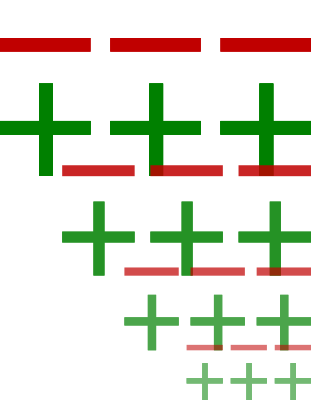
\includegraphics[width=0.2\paperwidth]{images/diffoscope_logo.png}
  };
 \end{tikzpicture}%
}
\begin{frame}{diffoscope}
 \frametitle{Debugging problems: diffoscope}

 \begin{itemize}
  \item Examines differences \textbf{in depth}
  \item Outputs HTML or plain text showing the differences
  \item Recursively unpacks archives
  \item Seeks human readability:
   \begin{itemize}
    \item uncompresses PDF
    \item disassembles binaries
    \item unpacks Gettext files
    \item … \textit{easy to extend to new file formats}
   \end{itemize}
  \item Falls back to binary comparison
  \item Entering stretch today!
 \end{itemize}
 \vfill
 \begin{center}
  \url{http://diffoscope.org/}\\
  {\footnotesize \color{gray}{(formely known as \texttt{debbindiff})}}
 \end{center}
\end{frame}
}

\begin{frame}
 \frametitle{diffoscope example (HTML output)}

 \begin{center}
  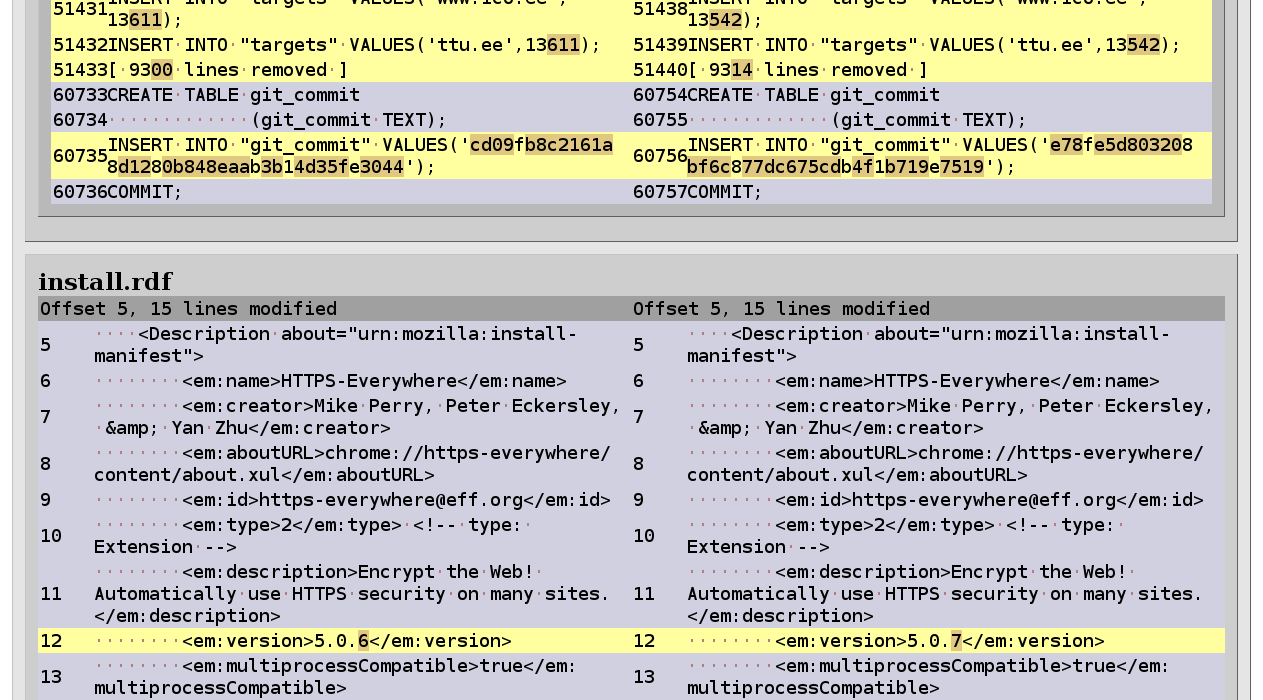
\includegraphics[width=0.9\paperwidth]{images/diffoscope_example_html.png}
 \end{center}
\end{frame}

\begin{frame}
 \frametitle{diffoscope example (text output)}

 \begin{center}
  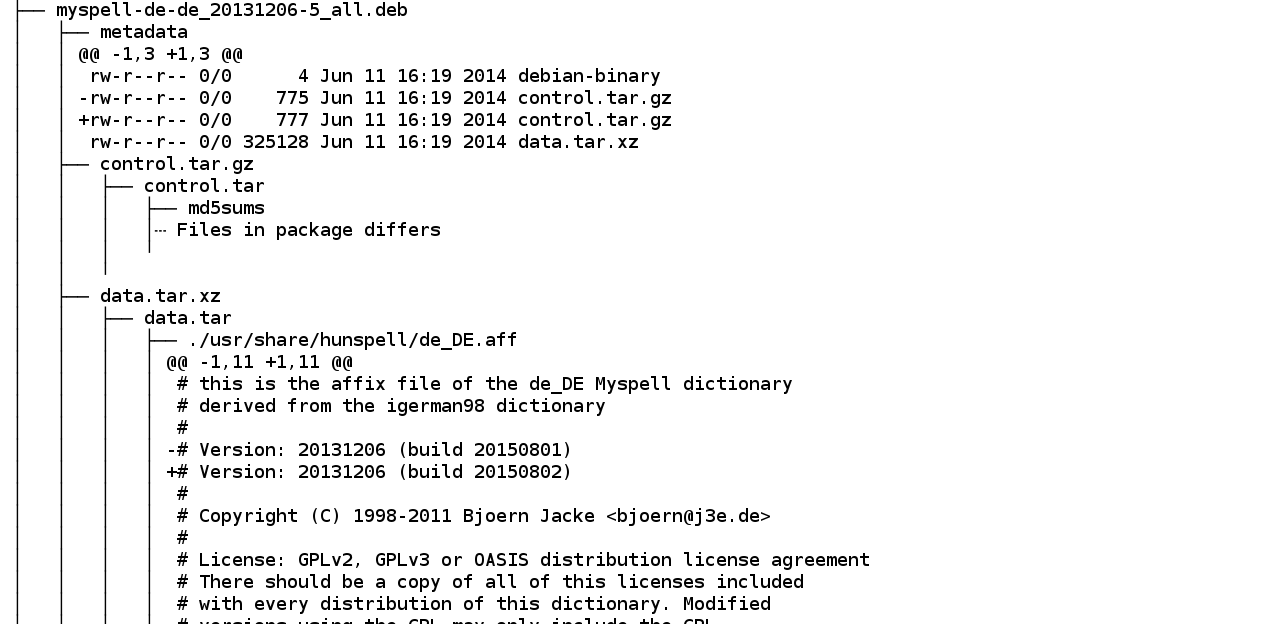
\includegraphics[width=0.9\paperwidth]{images/diffoscope_example_text.png}
 \end{center}
\end{frame}

\begin{frame}
 \frametitle{\texttt{SOURCE\_DATE\_EPOCH}}

 \begin{itemize}
  \item Build date usually not useful for the user
  \item Standardize a build-time environment variable
  \item (packages) When embedding current date, replace it by \texttt{SOURCE\_DATE\_EPOCH} if the env var is set
  \item General solution for other free software projects and distributions
  \item In Debian we set it to the latest debian/changelog entry timestamp
 \end{itemize}
\end{frame}

\begin{frame}
 \frametitle{\texttt{SOURCE\_DATE\_EPOCH} (closed bugs)}

 \begin{itemize}
  \item \texttt{\#787444} help2man
  \item \texttt{\#790899} epydoc
  \item \texttt{\#794004} ghostscript
  \item \texttt{\#783475} texi2html
  \item sphinx \small{\url{https://github.com/sphinx-doc/sphinx/pull/1954}}
 \end{itemize}

\end{frame}

\begin{frame}
 \frametitle{\texttt{SOURCE\_DATE\_EPOCH} (open bugs)}

 \begin{itemize}
  \item \texttt{\#792201} doxygen
  \item \texttt{\#790801} txt2man
  \item \texttt{\#791815} libxslt
  \item \texttt{\#792687} gettext (xgettext)
  \item \texttt{\#794681} qt4-x11 (qthelpgenerator)
  \item \texttt{\#794586} ocamldoc
  \item \texttt{\#792202} texlive-bin
  \item gcc (\texttt{\_\_DATE\_\_} and \texttt{\_\_TIME\_\_} macros) \texttt{\footnotesize{\url{https://gcc.gnu.org/ml/gcc-patches/2015-06/msg02210.html}}}
 \end{itemize}

\end{frame}

\section{Next?}

\begin{frame}
 \frametitle{dpkg}

 \begin{itemize}\small
  \item \sout{\texttt{\#719844}: make compression of \{data,control\}.tar.gz deterministic}
  \item \texttt{\#759999}: set reproducible timestamps in \texttt{.deb} ar file headers
  \item \texttt{\#787980}: normalize file permissions when creating control.tar
  \item \texttt{\#719845}: make file order within {data,control}.tar.gz deterministic
  \item \texttt{dpkg-genbuldinfo}: \textit{patch already written, but waiting on agreement about spec}
 \end{itemize}
\end{frame}

\begin{frame}
 \frametitle{debhelper}

 \begin{itemize}\small
  \item \texttt{\#759886}: make mtimes of packaged files deterministic
  \item \texttt{\#759895}: add a call to \texttt{dh\_strip\_nondeterminism} in \texttt{dh}
  \item \texttt{\#791823}: set \texttt{SOURCE\_DATE\_EPOCH} env var for reproducible builds
 \end{itemize}
\end{frame}

\begin{frame}
 \frametitle{cdbs}

 \begin{itemize}\small
  \item \texttt{\#794241}: export \texttt{\$SOURCE\_DATE\_EPOCH} to produce reproducible output
 \end{itemize}
\end{frame}

\begin{frame}
 \frametitle{sbuild}

 \begin{itemize}\small
  \item \texttt{\#790868}: allow sbuild to use a deterministic build path to build packages
  \item \texttt{\#778571}: predictible build location for reproducible builds
  \item Finish the \texttt{srebuild} script
 \end{itemize}
\end{frame}

\begin{frame}
 \frametitle{ftp.debian.org}

 \begin{itemize}\small
  \item \texttt{\#763822}: please include .buildinfo file in the archive
 \end{itemize}
\end{frame}


\begin{frame}{Fixing reproducibility issues}
 \begin{center}
  \Large
  Some examples
 \end{center}
\end{frame}

% Straightforward..

\begin{frame}{Timestamps in gzip headers}
 \begin{center}
  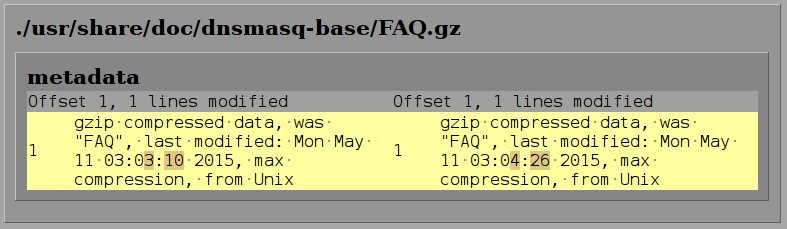
\includegraphics[width=0.9\textwidth]{images/examples/timestamps_in_gzip.png}
  \vfill
  \texttt{gzip FAQ} $\Longrightarrow$ \texttt{gzip -n FAQ}
 \end{center}
\end{frame}

\begin{frame}{Timestamps in Python version}
 \begin{center}
  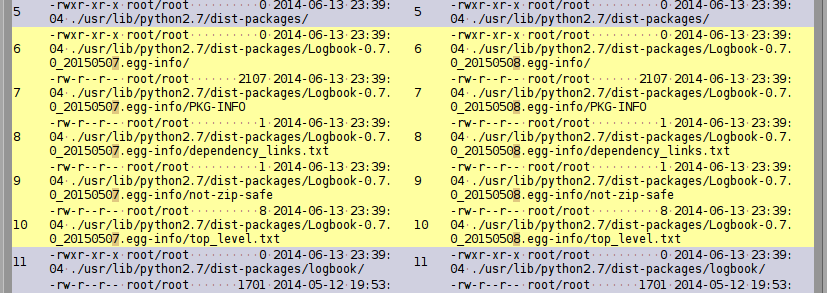
\includegraphics[width=0.9\textwidth]{images/examples/timestamps_in_python_version.png}
  \vfill
  \texttt{tag\_date=True} in \texttt{setup.py} $\Longrightarrow$ \texttt{tag\_date=False}
 \end{center}
\end{frame}


\begin{frame}{Timestamps in static libraries (cont.)}
 \begin{center}
  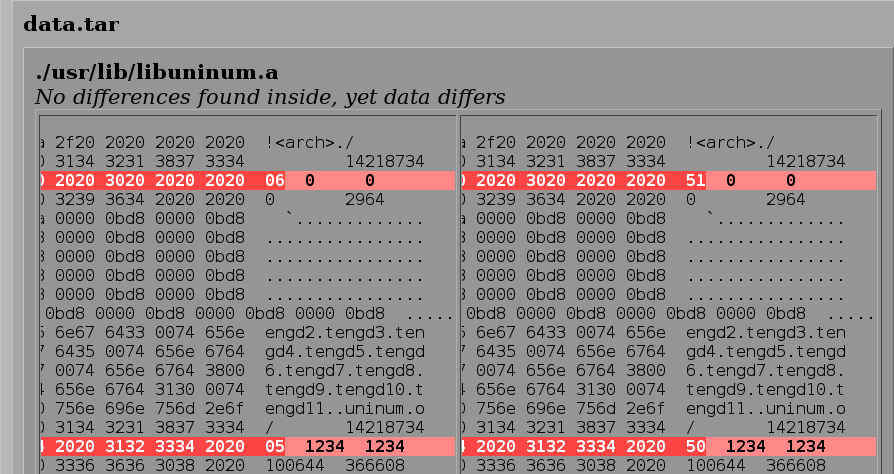
\includegraphics[width=0.9\textwidth]{images/examples/timestamps_in_static_library.png}
  \vfill
  \texttt{.a} files are \texttt{ar} archives $\Longrightarrow$ use \texttt{binutils} in determinstic mode or \texttt{strip-nondeterminism}
 \end{center}
\end{frame}

\begin{frame}{Timestamps in ZIP archives}
 \begin{center}
  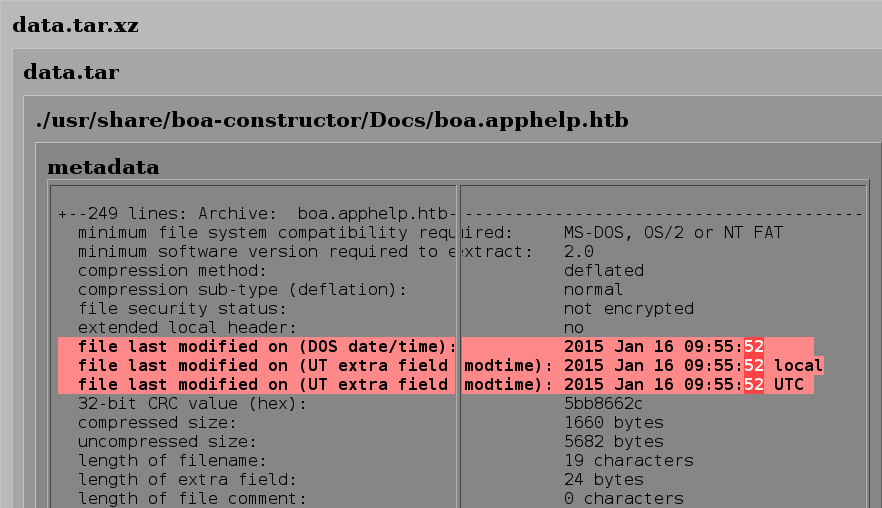
\includegraphics[width=0.9\textwidth]{images/examples/timestamps_in_zip.png}
  \vfill
  $\Longrightarrow$ \texttt{find}/\texttt{xargs}/\texttt{touch} to set mtime from \texttt{dpkg-parsechangelog} or \texttt{strip-nondeterminism}
 \end{center}
\end{frame}

\begin{frame}{Timestamps in Java jar}
 \begin{center}
  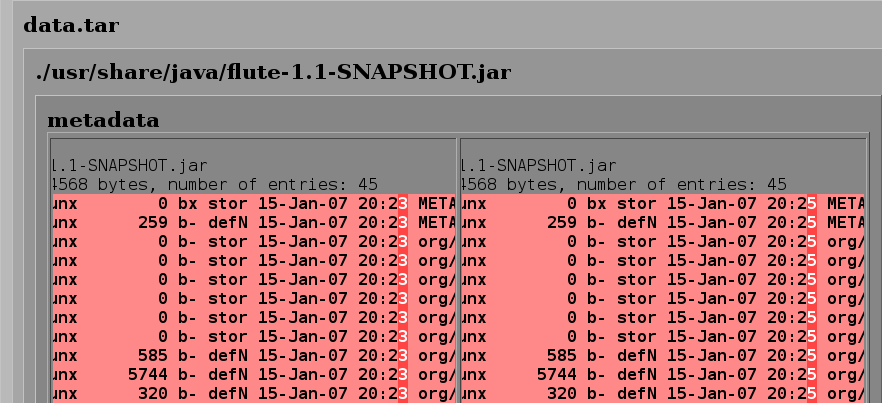
\includegraphics[width=0.9\textwidth]{images/examples/timestamps_in_jar.png}
  \vfill
  They are actually ZIP archives.
 \end{center}
\end{frame}

\begin{frame}{Timestamps written by Doxygen}
 \begin{center}
  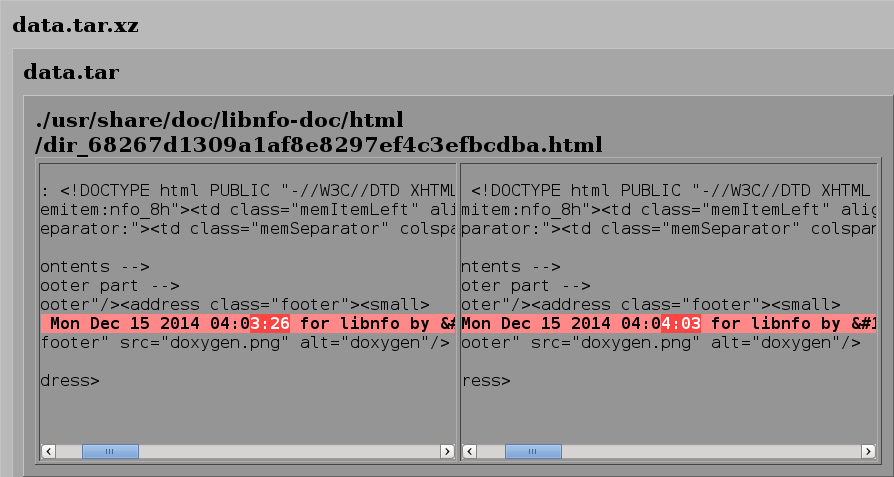
\includegraphics[width=0.9\textwidth]{images/examples/timestamps_by_doxygen.png}
  \vfill
  \texttt{HTML\_TIMESTAMP=NO}
 \end{center}
\end{frame}

\begin{frame}{Timestamps in tarballs}
 \begin{center}
  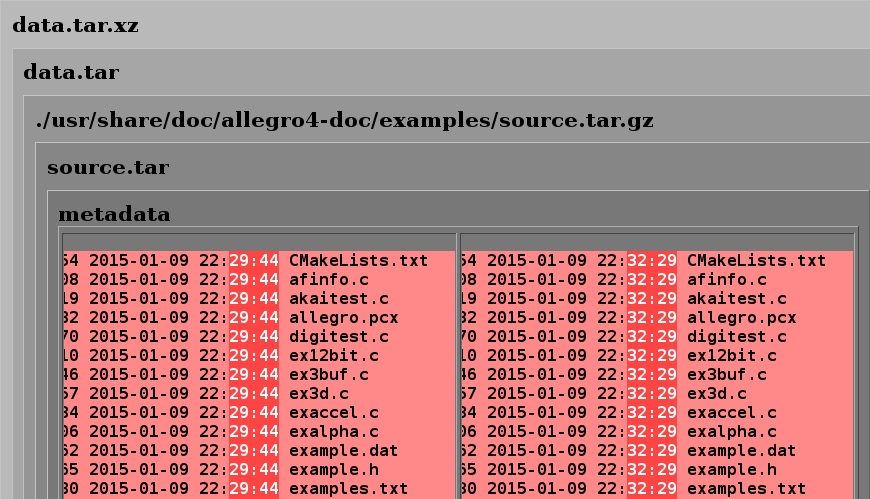
\includegraphics[width=0.9\textwidth]{images/examples/timestamps_in_tarball.png}
  \vfill
  \texttt{--mtime} to set all mtimes or adjust with \texttt{find}/\texttt{xargs}/\texttt{touch}
 \end{center}
\end{frame}

\begin{frame}{Users and groups in tarballs}
 \begin{center}
  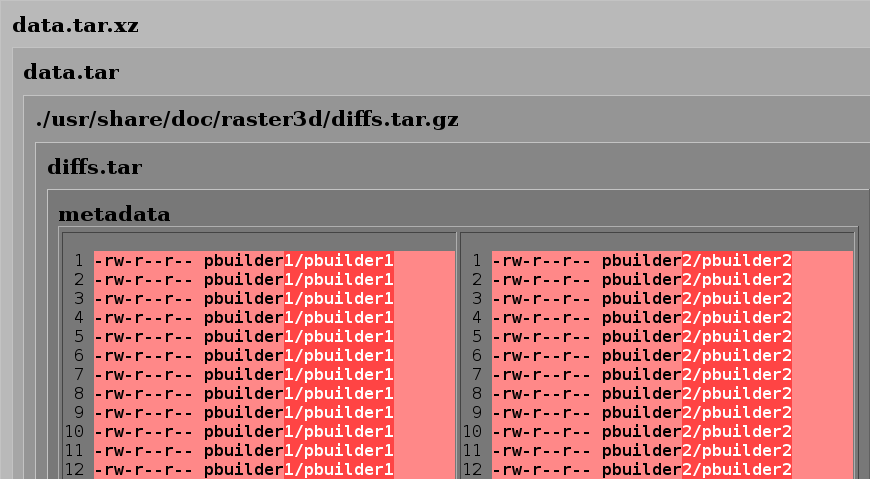
\includegraphics[width=0.9\textwidth]{images/examples/user_and_group_in_tarball.png}
  \vfill
  \texttt{--owner=root --group=root --numeric-owner}
 \end{center}
\end{frame}

\begin{frame}{Random order in tarballs}
 \begin{center}
  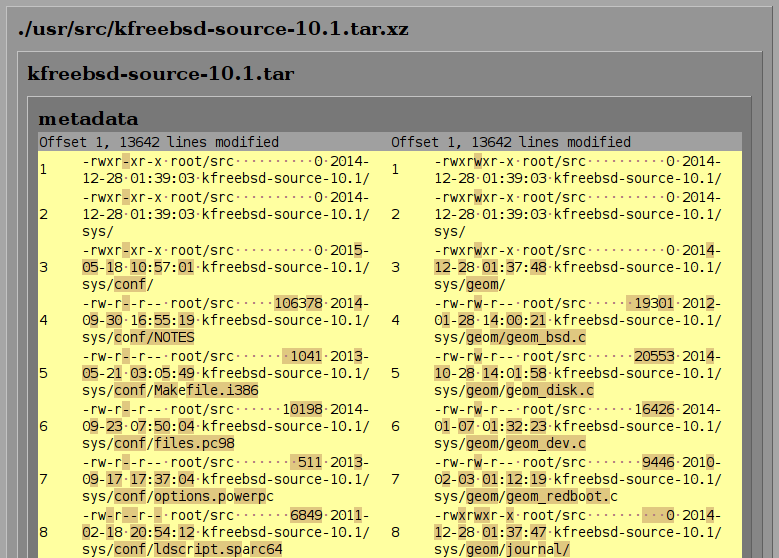
\includegraphics[width=0.7\textwidth]{images/examples/random_order_in_tarball.png}
  \vfill
  \texttt{find -type f | LC\_ALL=C sort | tar ...}
 \end{center}
\end{frame}

\begin{frame}{Timestamps in PNG}
 \begin{center}
  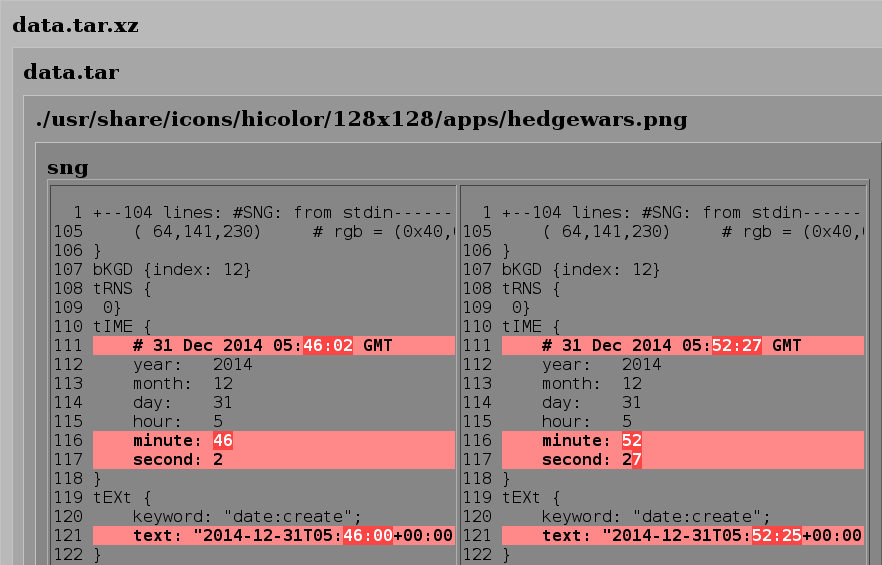
\includegraphics[width=0.9\textwidth]{images/examples/timestamps_in_png.png}
  \vfill
  \texttt{convert ... +set date:create +set date:modify -define png:exclude-chunk=time}
 \end{center}
\end{frame}

% toolchain

\begin{frame}{Timestamps written by Erlang compiler}
 \begin{center}
  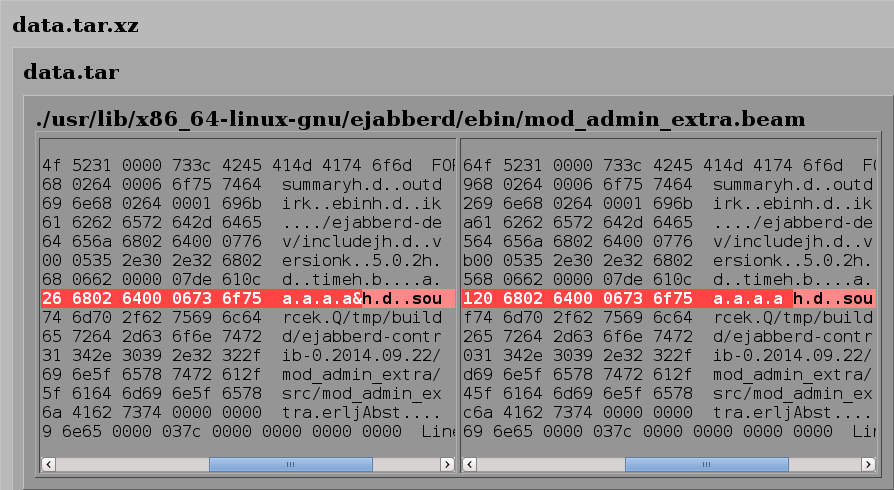
\includegraphics[width=0.9\textwidth]{images/examples/timestamps_in_beam.png}
  \vfill
  \vfill
  Patch \texttt{erlc} to obey \texttt{SOURCE\_DATE\_EPOCH} (\texttt{\#795834})
 \end{center}
\end{frame}

\begin{frame}{Timestamps in Ruby gemspec files}
 \begin{center}
  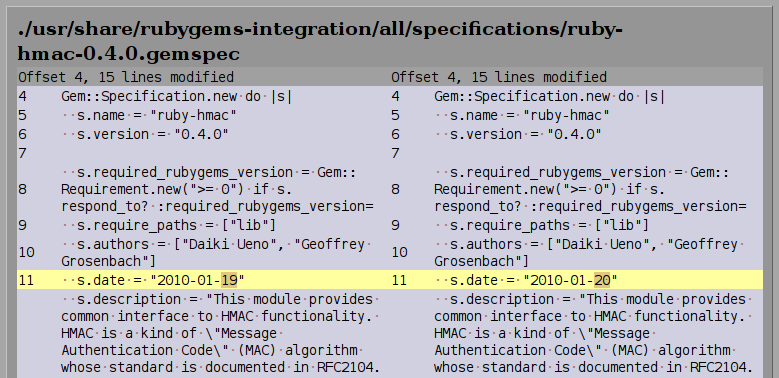
\includegraphics[width=0.9\textwidth]{images/examples/timestamps_in_ruby_gemspec.png}
  \vfill
  Varies on timezone $\Longrightarrow$ patch to always use UTC (\texttt{\#779631})
 \end{center}
\end{frame}

\begin{frame}{Timestamps written by docbook-to-man}
 \begin{center}
  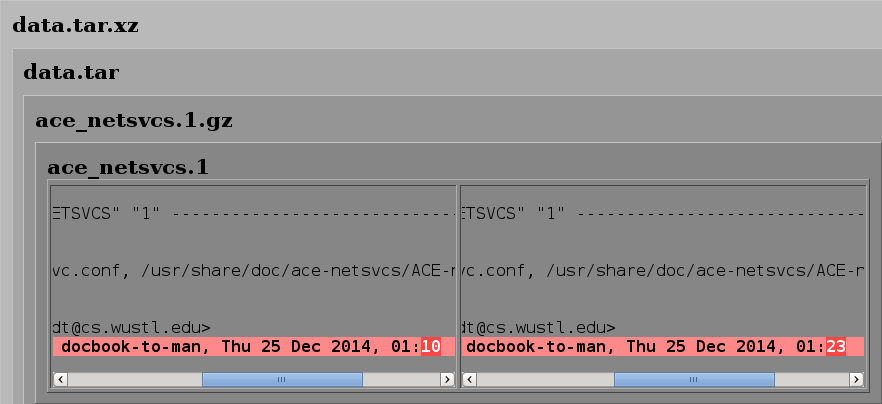
\includegraphics[width=0.9\textwidth]{images/examples/docbook-to-man.png}
  \vfill
  Fix docbook-to-man (\texttt{\#776143})
 \end{center}
\end{frame}

% ugly

\begin{frame}{Hostname / build time recorded via ./configure}
 \begin{center}
  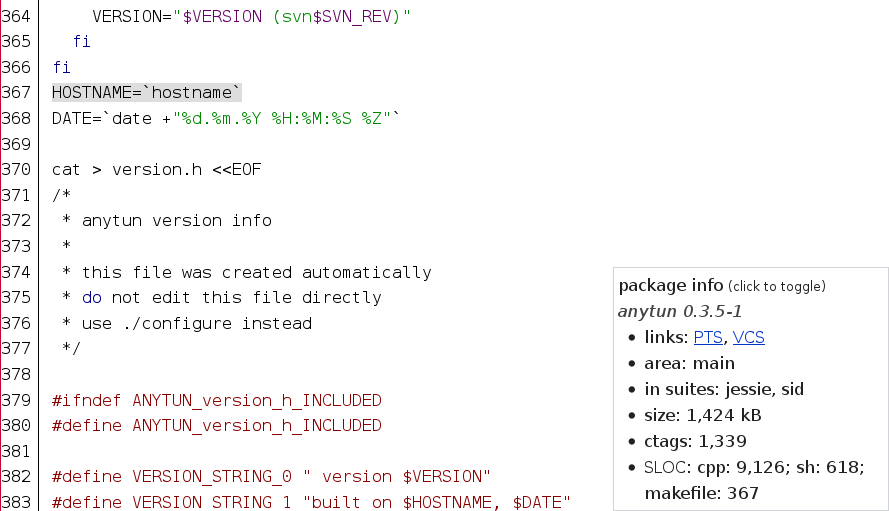
\includegraphics[width=0.9\textwidth]{images/examples/hostname_in_configure.png}
  \vfill
  Maybe override in \texttt{debian/rules}..?
 \end{center}
\end{frame}

% uglier

\begin{frame}{Timestamps in header files}
 \begin{center}
  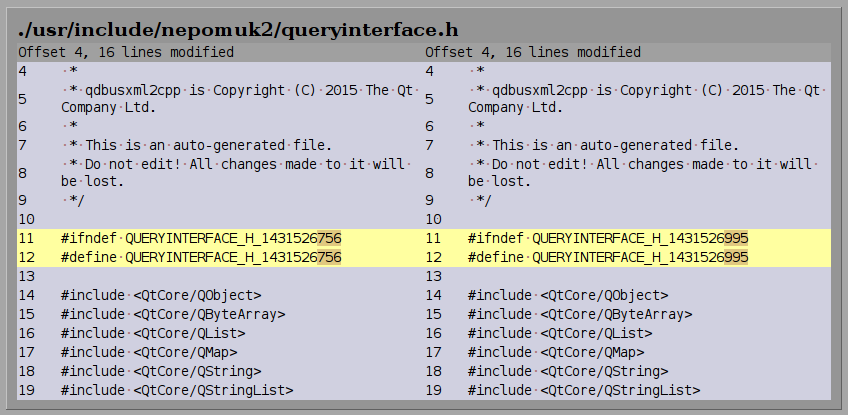
\includegraphics[width=0.9\textwidth]{images/examples/timestamps_in_header_files.png}
  \vfill
  Patch with a better unique id or use \texttt{SOURCE\_DATE\_EPOCH}
 \end{center}
\end{frame}

\begin{frame}{Recorded kernel version}
 \begin{center}
  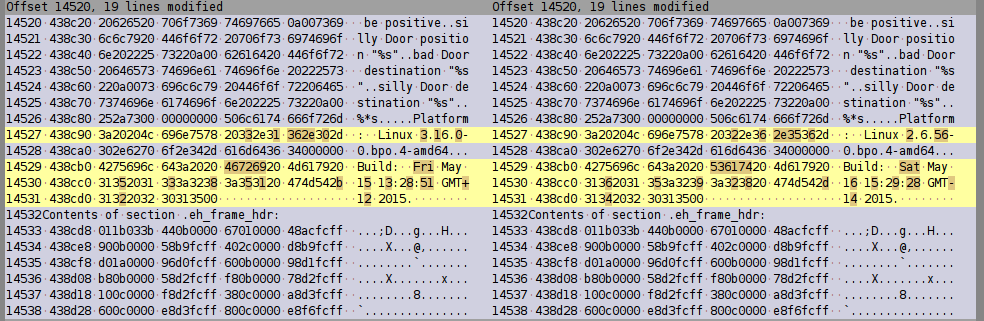
\includegraphics[width=0.9\textwidth]{images/examples/embedded_kernel_version.png}
  \vfill
  Privacy leak! $Longrightarrow$ Patch upstream
 \end{center}
\end{frame}

\begin{frame}{Build time recorded via Makefile}
 \begin{center}
  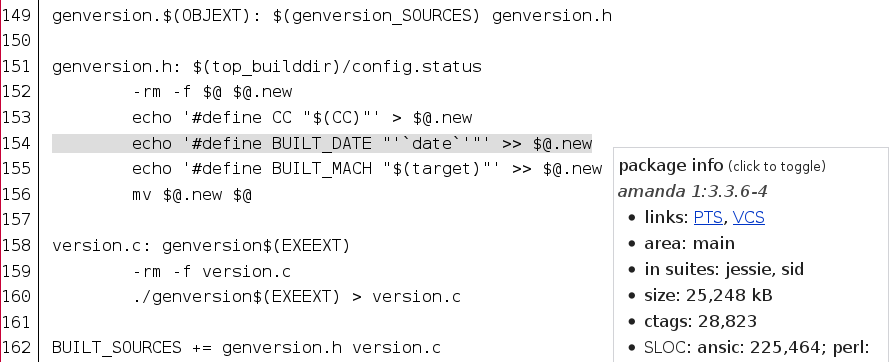
\includegraphics[width=0.9\textwidth]{images/examples/build_date_in_makefile.png}
  \vfill
  Patch upstream.
 \end{center}
\end{frame}

\begin{frame}
 \frametitle{Toolchain work}

 % list taken from https://wiki.debian.org/ReproducibleBuilds/ExperimentalToolchain on 2015-08-19
 % Skipping SOURCE_DATE_EPOCH related patches since they are listed in the related section
 \begin{itemize}\small
  \item \sout{\texttt{\#776026} \textbf{wheel:} create reproducible wheel (.whl) files}
  \item \sout{\texttt{\#776143} \textbf{docbook-to-man:} remove timestamps from the generated manpages}
  \item \sout{\textbf{gtk-doc:} generate its links in a stable order}
  \item \texttt{\#774148} \textbf{fontforge:} propagate creation and modification times from source file
  \item \texttt{\#775786} \textbf{python-support:} sort file lists in /usr/share/python-support/*.private
  \item \textbf{libxslt:} make generate-id() return identifiers in a deterministic way
  \item And many more! \url{https://deb.li/3bX6F}
 \end{itemize}
\end{frame}

\begin{frame}
 \frametitle{Individual packages}

 \begin{itemize}
  \item 644 bugs for individual problems
  \item 610 tagged “patch”
  \item Nearly two patches per day since Fall 2014 on average!
 \end{itemize}
\end{frame}

\begin{frame}[plain]
 \begin{tikzpicture}[remember picture,overlay]
  \node[at=(current page.center)] {
    \includegraphics[width=\paperwidth]{images/stats_pkg_state.png}
  };
 \end{tikzpicture}
\end{frame}

\begin{frame}[plain]
 \begin{tikzpicture}[remember picture,overlay]
  \node[at=(current page.center)] {
    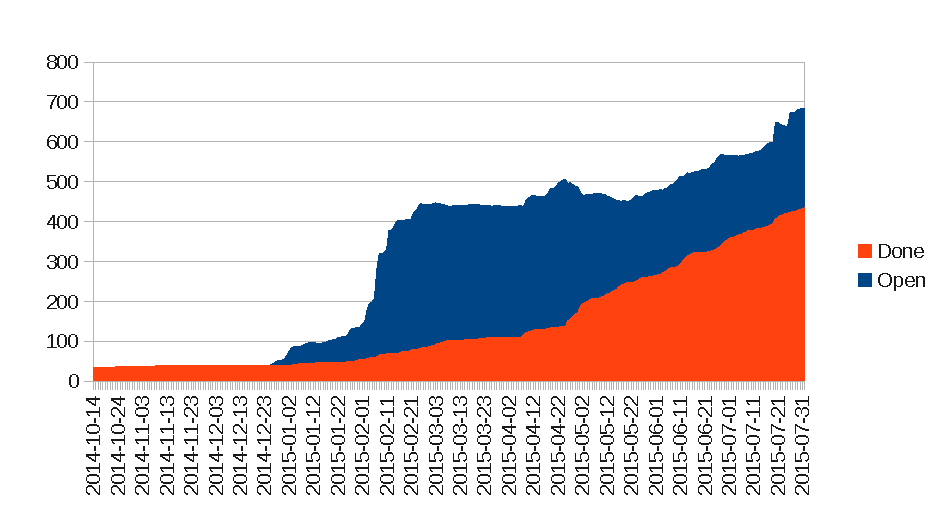
\includegraphics[width=\paperwidth]{images/bug_chart.pdf}
  };
 \end{tikzpicture}
\end{frame}

\begin{frame}
 \frametitle{Debian policy}

 \begin{itemize}
  \item Section 4.15: “Source must build in a reproducible manner”? 
 \end{itemize}
\end{frame}

\section{Want to help?}

\begin{frame}
 \frametitle{Fix your package}

 \begin{center}
  \texttt{https://reproducible.debian.net/\textit{package}}

  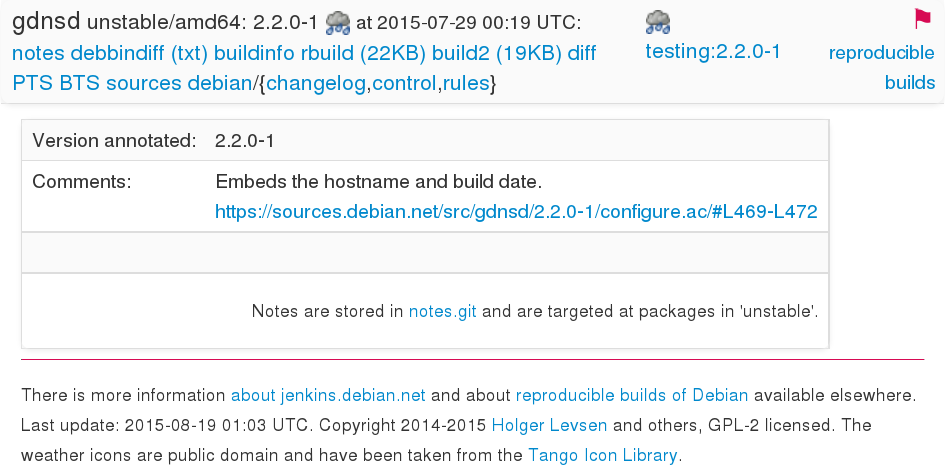
\includegraphics[width=\linewidth]{images/rdn-gdnsd.png}
 \end{center}
\end{frame}

\begin{frame}
 \frametitle{Fix your package}

 \begin{center}
  \texttt{https://tracker.debian.org/\textit{package}}

  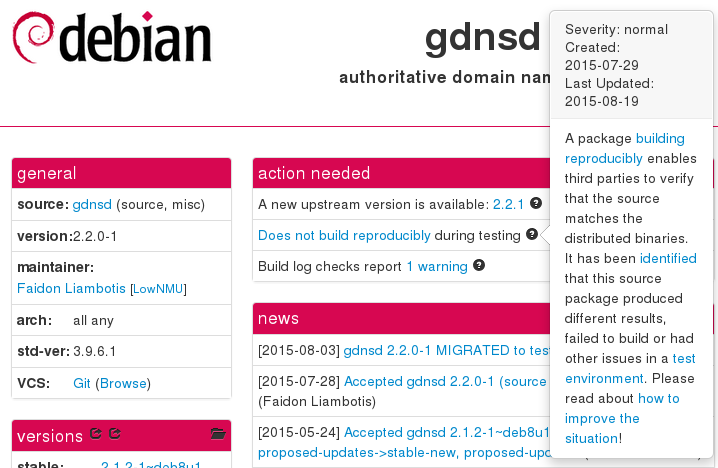
\includegraphics[width=0.8\linewidth]{images/tracker-gdnsd.png}
 \end{center}
\end{frame}

\begin{frame}
 \frametitle{Fix your package}

 \begin{itemize}
  \item And also:
   \begin{itemize}
    \item DDPO
    \item DMD
   \end{itemize}
  \item Tips on the wiki \\
   {\small \url{https://wiki.debian.org/ReproducibleBuilds/Howto}}
  \item Ask for help on \texttt{\#debian-reproducible} \\
   or on the mailing-list
 \end{itemize}
\end{frame}

\begin{frame}
 \frametitle{Fix your package}

 \begin{itemize}
  \item Testing:
   \begin{itemize}
    \item Requires \texttt{pbuilder} and custom config
    \item Need the “reproducible” repository
    \item Documented on the wiki
    \item diffoscope is in \textit{unstable}
   \end{itemize}
  \item Addition to \texttt{devscripts} once \texttt{dpkg} is good
  \item Come to the hack session! \\
    2015-08-21 14:00..19:00 in Stockholm
 \end{itemize}
\end{frame}

\begin{frame}
 \frametitle{Join the team!}

 \begin{itemize}
  \item Why?
   \begin{itemize}
    \item \heartsuit{}\heartsuit{}\heartsuit{} Lovely group of people \heartsuit{}\heartsuit{}\heartsuit{}
    \item Learn something new everyday
    \item Change the (software) world!
   \end{itemize}
  \item What do we do?
   \begin{itemize}
    \item Review packages
    \item Identify issues and document solutions
    \item \texttt{reproducible.d.n}, diffoscope, strip-nondeterminism
    \item Propose changes for toolchain
    \item Submit patches for individual packages
    \item Write more general documentation and  talk to the world
   \end{itemize}
 \end{itemize}
\end{frame}

\section{Questions?}

\begin{frame}
 \frametitle{Thanks!}

 \begin{itemize}
  \item You and everybody who contributed!
  \item Linux Foundation and the Core Infrastructure Initiative
 \end{itemize}

 \begin{center}
  
\includegraphics[height=0.1\paperheight]{images/linux_foundation_logo.png}
  \hspace{0.1\paperwidth}
  
\includegraphics[height=0.1\paperheight]{images/cii_logo.png}
 \end{center}

 \vfill
 \begin{center}
  \resizebox{0.8\textwidth}{!}{%
   \begin{tabular}{rl}
    \texttt{lunar@debian.org} & \texttt{0603 CCFD 9186 5C17 E88D} \\
                              & \texttt{4C79 8382 C95C 2902 3DF9} \\
    \texttt{holger@debian.org} & \texttt{B8BF 5413 7B09 D35C F026} \\
                               & \texttt{FE9D 091A B856 069A AA1C} \\
    \texttt{lamby@debian.org} & \texttt{C2FE 4BD2 71C1 39B8 6C53} \\
                              & \texttt{3E46 1E95 3E27 D431 1E58} \\
    \texttt{dhole@openmailbox.org} & \texttt{9BC4 8EF8 08DB 91DD 158D} \\
                                   & \texttt{559D 4FA4 57A1 8514 CC63}
   \end{tabular}
  }
 \end{center}
\end{frame}

\end{document}
